%%%%%%%%%%%%%%%%%%%%%%%%%%%%%%%%%%%%%%%%%
% Programming/Coding Assignment
% LaTeX Template
%
% This template has been downloaded from:
% http://www.latextemplates.com
%
% Original author:
% Ted Pavlic (http://www.tedpavlic.com)
%
% Note:
% The \lipsum[#] commands throughout this template generate dummy text
% to fill the template out. These commands should all be removed when 
% writing assignment content.
%
% This template uses a Perl script as an example snippet of code, most other
% languages are also usable. Configure them in the "CODE INCLUSION 
% CONFIGURATION" section.
%
%Assignment 6
%Author Zetan
%%%%%%%%%%%%%%%%%%%%%%%%%%%%%%%%%%%%%%%%%

%----------------------------------------------------------------------------------------
%	PACKAGES AND OTHER DOCUMENT CONFIGURATIONS
%----------------------------------------------------------------------------------------

\documentclass{article}

\usepackage{fancyhdr} % Required for custom headers
\usepackage{lastpage} % Required to determine the last page for the footer
\usepackage{extramarks} % Required for headers and footers
\usepackage[usenames,dvipsnames]{color} % Required for custom colors
\usepackage{graphicx} % Required to insert images
\usepackage{listings} % Required for insertion of code
\usepackage{courier} % Required for the courier font
\usepackage{multirow}
\usepackage{listings,multicol}
\usepackage{pgfplots,pgfplotstable}
 \usepackage{amssymb}

\usepackage{url}

% Margins
\topmargin=-0.45in
\evensidemargin=0in
\oddsidemargin=0in
\textwidth=6.5in
\textheight=9.0in
\headsep=0.25in

\linespread{1.1} % Line spacing

% Set up the header and footer
\pagestyle{fancy}
\lhead{\hmwkAuthorName} % Top left header
\chead{\hmwkClass\ (\hmwkClassInstructor\ \hmwkClassTime): \hmwkTitle} % Top center head
\rhead{\firstxmark} % Top right header
\lfoot{\lastxmark} % Bottom left footer
\cfoot{} % Bottom center footer
\rfoot{Page\ \thepage\ of\ \protect\pageref{LastPage}} % Bottom right footer
\renewcommand\headrulewidth{0.4pt} % Size of the header rule
\renewcommand\footrulewidth{0.4pt} % Size of the footer rule

\setlength\parindent{0pt} % Removes all indentation from paragraphs

%----------------------------------------------------------------------------------------
%	CODE INCLUSION CONFIGURATION
%----------------------------------------------------------------------------------------
\definecolor{lightgray}{rgb}{.9,.9,.9}
\definecolor{darkgray}{rgb}{.4,.4,.4}
\definecolor{purple}{rgb}{0.65, 0.12, 0.82}
\definecolor{MyDarkGreen}{rgb}{0.0,0.4,0.0} % This is the color used for comments
\lstloadlanguages{Python} % Load python syntax for listings, for a list of other languagesftp://ftp.tex.ac.uk/tex-archive/macros/latex/contrib/listings/listings.pdf supported see: 
\lstdefinelanguage{JavaScript}{
  keywords={break, case, catch, continue, debugger, default, delete, do, else, false, finally, for, function, if, in, instanceof, new, null, return, switch, this, throw, true, try, typeof, var, void, while, with},
  morecomment=[l]{//},
  morecomment=[s]{/*}{*/},
  morestring=[b]',
  morestring=[b]",
  ndkeywords={class, export, boolean, throw, implements, import, this},
  keywordstyle=\color{blue}\bfseries,
  ndkeywordstyle=\color{darkgray}\bfseries,
  identifierstyle=\color{black},
  commentstyle=\color{purple}\ttfamily,
  stringstyle=\color{red}\ttfamily,
  sensitive=true
}
\lstset{
        frame=single, % Single frame around code
        basicstyle=\small\ttfamily, % Use small true type font
        keywordstyle=[1]\color{Blue}\bf, % python functions bold and blue
        keywordstyle=[2]\color{Purple}, % python function arguments purple
        keywordstyle=[3]\color{Blue}\underbar, % Custom functions underlined and blue
        identifierstyle=, % Nothing special about identifiers                                         
        commentstyle=\usefont{T1}{pcr}{m}{sl}\color{MyDarkGreen}\small, % Comments small dark green courier font
        stringstyle=\color{Purple}, % Strings are purple
        showstringspaces=false, % Don't put marks in string spaces
        tabsize=5, % 5 spaces per tab
        breaklines=true,
        %
        % Put standard python functions not included in the default language here
        morekeywords={rand},
        %
        % Put python function parameters here
        morekeywords=[2]{on, off, interp},
        %
        % Put user defined functions here
        morekeywords=[3]{test},
       	%
        morecomment=[l][\color{Blue}]{...}, % Line continuation (...) like blue comment
        numbers=left, % Line numbers on left
        firstnumber=1, % Line numbers start with line 1
        numberstyle=\tiny\color{Blue}, % Line numbers are blue and small
        stepnumber=5 % Line numbers go in steps of 5
}

% Creates a new command to include a pyton script, the first parameter is the filename of the script (without .py), the second parameter is the caption
\newcommand{\pythonscript}[2]{
\begin{itemize}
\item[]\lstinputlisting[language=python,caption=#2,label=#1]{#1.py}
\end{itemize}
}
% Creates a new command to include a shell script, the first parameter is the filename of the script (without .sh), the second parameter is the caption
\newcommand{\shellscript}[2]{
\begin{itemize}
\item[]\lstinputlisting[language=bash,caption=#2,label=#1]{#1.sh}
\end{itemize}
}
% Creates a new command to include a R script, the first parameter is the filename of the script (without .R), the second parameter is the caption
\newcommand{\Rscript}[2]{
\begin{itemize}
\item[]\lstinputlisting[language=R,caption=#2,label=#1]{#1.R}
\end{itemize}
}
% Creates a new command to include a java script, the first parameter is the filename of the script (without .R), the second parameter is the caption
\newcommand{\jsscript}[2]{
\begin{itemize}
\item[]\lstinputlisting[language=JavaScript,caption=#2,label=#1]{#1.js}
\end{itemize}
}
%----------------------------------------------------------------------------------------
%	DOCUMENT STRUCTURE COMMANDS
%	Skip this unless you know what you're doing
%----------------------------------------------------------------------------------------

% Header and footer for when a page split occurs within a problem environment
\newcommand{\enterProblemHeader}[1]{
\nobreak\extramarks{#1}{#1 continued on next page\ldots}\nobreak
\nobreak\extramarks{#1 (continued)}{#1 continued on next page\ldots}\nobreak
}

% Header and footer for when a page split occurs between problem environments
\newcommand{\exitProblemHeader}[1]{
\nobreak\extramarks{#1 (continued)}{#1 continued on next page\ldots}\nobreak
\nobreak\extramarks{#1}{}\nobreak
}

\setcounter{secnumdepth}{0} % Removes default section numbers
\newcounter{homeworkProblemCounter} % Creates a counter to keep track of the number of problems

\newcommand{\homeworkProblemName}{}
\newenvironment{homeworkProblem}[1][Problem \arabic{homeworkProblemCounter}]{ % Makes a new environment called homeworkProblem which takes 1 argument (custom name) but the default is "Problem #"
\stepcounter{homeworkProblemCounter} % Increase counter for number of problems
\renewcommand{\homeworkProblemName}{#1} % Assign \homeworkProblemName the name of the problem
\section{\homeworkProblemName} % Make a section in the document with the custom problem count
\enterProblemHeader{\homeworkProblemName} % Header and footer within the environment
}{
\exitProblemHeader{\homeworkProblemName} % Header and footer after the environment
}

\newcommand{\problemAnswer}[1]{ % Defines the problem answer command with the content as the only argument
\noindent\framebox[\columnwidth][c]{\begin{minipage}{0.98\columnwidth}#1\end{minipage}} % Makes the box around the problem answer and puts the content inside
}

\newcommand{\homeworkSectionName}{}
\newenvironment{homeworkSection}[1]{ % New environment for sections within homework problems, takes 1 argument - the name of the section
\renewcommand{\homeworkSectionName}{#1} % Assign \homeworkSectionName to the name of the section from the environment argument
\subsection{\homeworkSectionName} % Make a subsection with the custom name of the subsection
\enterProblemHeader{\homeworkProblemName\ [\homeworkSectionName]} % Header and footer within the environment
}{
\enterProblemHeader{\homeworkProblemName} % Header and footer after the environment
}

%----------------------------------------------------------------------------------------
%	NAME AND CLASS SECTION
%----------------------------------------------------------------------------------------

\newcommand{\hmwkTitle}{Assignment\ \#6} % Assignment title
\newcommand{\hmwkDueDate}{Thursday,\ March\ 17,\ 2016} % Due date
\newcommand{\hmwkClass}{Web Science\ cs532} % Course/class
\newcommand{\hmwkClassTime}{4:20pm} % Class/lecture time
\newcommand{\hmwkClassInstructor}{Dr.Michael.L.Nelson} % Teacher/lecturer
\newcommand{\hmwkAuthorName}{Zetan Li} % Your name

%----------------------------------------------------------------------------------------
%	TITLE PAGE
%----------------------------------------------------------------------------------------

\title{
\vspace{2in}
\textmd{\textbf{\hmwkClass:\ \hmwkTitle}}\\
\normalsize\vspace{0.1in}\small{Due\ on\ \hmwkDueDate}\\
\vspace{0.1in}\large{\textit{\hmwkClassInstructor\ \hmwkClassTime}}
\vspace{3in}
}

\author{\textbf{\hmwkAuthorName}}
\date{} % Insert date here if you want it to appear below your name

%----------------------------------------------------------------------------------------

\begin{document}

\maketitle

%----------------------------------------------------------------------------------------
%	TABLE OF CONTENTS
%----------------------------------------------------------------------------------------

%\setcounter{tocdepth}{1} % Uncomment this line if you don't want subsections listed in the ToC

\newpage
\tableofcontents
\newpage

%----------------------------------------------------------------------------------------
%	PROBLEM 1
%----------------------------------------------------------------------------------------

% To have just one problem per page, simply put a \clearpage after each problem

\begin{homeworkProblem}
Use D3 to visualize your Twitter followers.  Use my twitter account
(``@phonedude\_mln") if you do not have \url{>=} 50 followers.  For example,
@hvdsomp follows me, as does @mart1nkle1n.  They also follow each
other, so they would both have links to me and links to each other.\\
\\
To see if two users follow each other, see:\\
\url{https://dev.twitter.com/rest/reference/get/friendships/show}\\
\\
Attractiveness of the graph counts!  Nodes should be labeled (avatar
images are even better), and edge types (follows, following) should
be marked.\\
\\
Note: for getting GitHub to serve HTML (and other media types), see:\\
\url{http://stackoverflow.com/questions/6551446/can-i-run-html-files-directly-from-github-instead-of-just-viewing-their-source}\\
\\
Be sure to include the URI(s) for your D3 graph in your report. \\
\\
\centerline{SOLUTION}
First, we have to get the followship data from twitter.\\
Tweepy have a function called api.show\_friendship which wraps the REST API for followship query.\\
\\
However, this query only allows a pair at a time, and twitter has the limit of 180 search terms per 18 minutes, the total query time is the combination of 2 out of total number of followers. So we have to minimize out data scale. \\
\\
Here, we pick the follower ``joc7188" as our test case. He's user name is Jose Antonio Olvera and he has 52 followers since we inspect his account.\\
To get the network graph of his follower, first we have to get all his follower accounts.\\
Below is the code to extract all his followers.\\
\pythonscript{p1_getlist}{Python script to get all follower accounts}
Now we have the list of all his followers. Next step is to inspect the followship between them.\\
\\
api.show\_friendship returns a tuple contains two friendship objects, which represent state of friendship of two account we queried. We can get ``following'' and ``followed\_by'' from either of them. \\
\\
Due to the rate limit of the twitter, this takes a long time to get all the data.\\
\pythonscript{p1_getfriendship}{Python script to get followship between followers}
Right now, we have all the data we need to plot the d3 graph.\\
We could use d3.tsv to parse the file which separated by tab.\\
To build the links, we have to iterate each link in our data file, add link according to the link type. (In our data file, we defined 0 as following, 1 as followed by, and 2 as bidirectional following)\\
Then add each node to the graph and plot a curve \cite{curve} on each link (special thanks to rcond for his code inspired me on how to plot the markers).\\
\jsscript{twitter}{Core code to construct the d3 graph}
Below is the d3 graph screen capture, for online rendering, see \url{https://rawgit.com/DarkAngelZT/cs532-s16/master/assignments/a6/d3/twitter.html}
\begin{figure}
\centering
\caption{d3 graph}
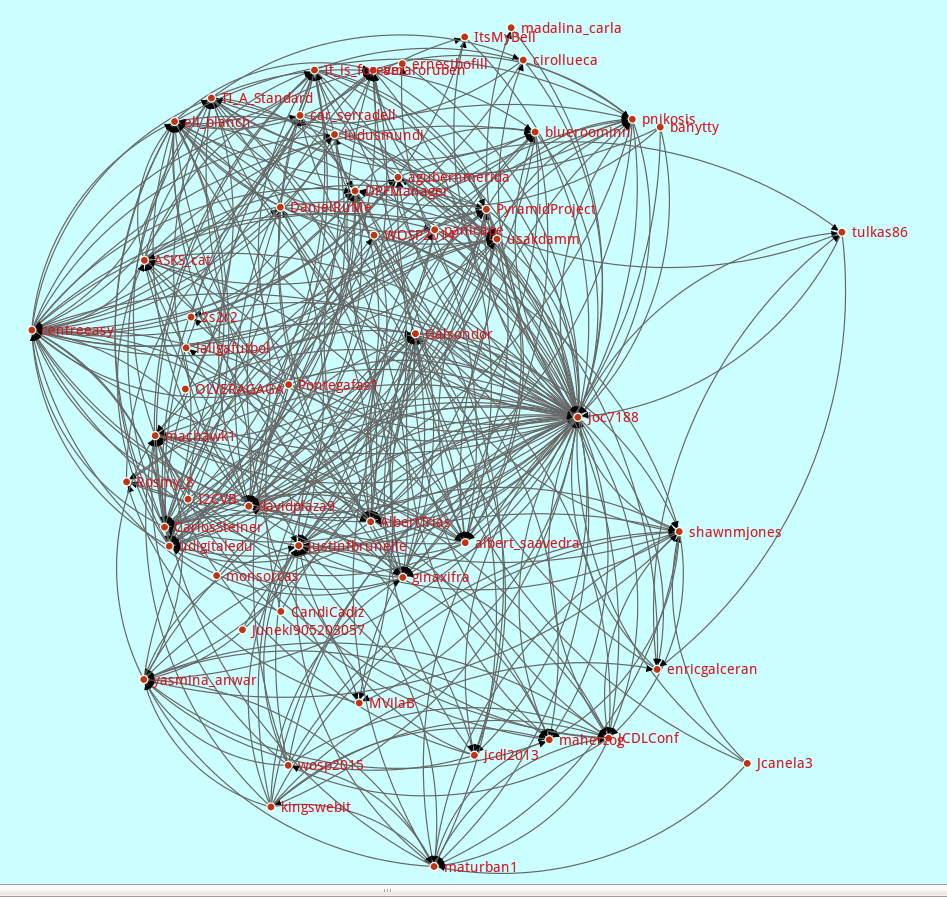
\includegraphics[scale=0.55]{p1.png}
\end{figure}
\end{homeworkProblem}
\pagebreak
%----------------------------------------------------------------------------------------
%	PROBLEM 2
%----------------------------------------------------------------------------------------
\begin{homeworkProblem}
Take the Twitter graph you generated in question \#1 and test for
male-female homophily.  For the purposes of this question you can
consider the graph as undirected (i.e., no distinction between 
``follows" and ``following").  Use the twitter name (not ``screen
name"; for example ``Michael L. Nelson" and not ``@phonedude\_mln")
and programatically determine if the user is male or female.  Some
sites that might be useful:\\
\\
\url{https://genderize.io/}\\
\url{https://pypi.python.org/pypi/gender-detector/0.0.4}\\
\\
Create a table of Twitter users and their likely gender.  List any 
accounts that can't be determined and remove them from the graph.\\
\\
Perform the homophily test as described in slides 11-15, Week 7.\\
\\
Does your Twitter graph exhibit gender homophily?\\
\\
\centerline{SOLUTION}
Since we have all the follower's account, It's easy to get their possible gender.\\
So far in our dataset, only the screen name is recorded. We have to get their real name first. Using api.get\_user, then we can retrieve user name in the field called``user.name''.
\pythonscript{p2_getname}{Python script to get user names}
Then we can use online service genderize.io to get their possible gender.\cite{gender}\\
Algorithm is like this:\\
1) Pair each account name and user name then get their gender via genderize.io, store all of them into data file.\\
2) Look up every link in the followship data table.\\
3) Extract two account name from each followship.\\
4) Look up their user name and get the gender from data file.\\
5) If two genders are different, mark them as a cross gender link.\\
6) Repeat 2) to 5) until all the links are analyzed.\\
Below is the script implement:
\pythonscript{p2_gender}{Python script to get gender of each account}
Some names are too confusing to guess, so these account are dropped:
\lstinputlisting[ multicols=2,breaklines=true]{p2_dropped.txt}
The gender list we have:
\\
\pgfplotstableread[comment chars={E}, col sep=tab]{gender.txt}\mytable
\pgfplotstabletypeset[
string type,header=false,
after row={\hline},
] {\mytable}
\\
Finally, calculate the male and female numbers to perform the homophily test.
\pythonscript{p2_crossgender}{python code to test the gender homophily}
Below is the script output:\\
\lstinputlisting[ breaklines=true]{p2_gender_homophily.txt}
From above, we can see the percentage of cross gender edge is 0.31 < 2pq,
$\therefore$ Evidence of homophily
\end{homeworkProblem}
\bibliographystyle{plain}
\bibliography{ref}
\end{document}